\chapter{New library with Complete contracts}
\label{sec:LibraryDesign}

One part of this semester thesis was the redesign of the EiffelBase Library (cf. \cite{eiffelbase}). The goal was to get a cleaner and smoother base library. The new base library should use Dynamic Frame Contracts and Models as discussed in Section \ref{sec:DynamicFramesInEiffel} and Section \ref{sec:ModelsInEiffel}. The redesign was focused on LINKED\_LIST class and all supporting classes.

The current EiffelBase Library is over engineered and sometimes messy. Some features have names which do not comply with the own Eiffel style guidelines (cf. Chapter 26 in \cite{Meyer97Object}) or which do not reflect the true meaning of this feature or even of a class. An example for this is cursor which in Eiffel is rather a cursor position rather than a real cursor.

\section{EiffelBase with Complete Contracts}
\label{sec:EiffelBaseWithCompleteContracts}

As stated above the new base library was focused on the LINKED\_LIST class and all supporting classes. In total there are about 20 classes in the library. Every class has a `CC\_' prefix in front of the name to be able to use this library in parallel to the original EiffelBase Library.

\subsection{Differences to EiffelBase}
\label{sec:DifferencesToEiffelBase}

Actually there are a lot of differences to the original EiffelBase Library. We try to give a short overview over these changes and explain the basic concepts and ideas that led to these differences.

\begin{description}
	\item [Finite containers] In contrast to the EiffelBase Library the new library is always finite. To be more precise, only finite containers are available.
	\item [TABLE not a heir of BAG] The TABLE class is no longer a heir of the BAG class. Originally in the EiffelBase Library the idea was that a table is a bag of elements which can be directly accessed through an index. But for us the mathematical concept behind a bag and a table are too different to be directly related.
	\item [ACTIVE not a heir of BAG] The ACTIVE class is no longer a heir of the BAG class. An active object is defined as a data structure, which at every stage has a possibly undefined current item. Here again the mathematical concept behind an active and a bag are too different to be directly related.
	\item [INDEXABLE not a heir of TABLE] The INDEXABLE class is no longer a heir of the TABLE class.
	\item [Feature renaming] Some features in the original EiffelBase Library have names which do not reflect the actual meaning or which are not compliant with the Eiffel style guidelines (cf. Chapter 26 in \cite{Meyer97Object}).
	\begin{itemize}
		\item Feature cursor in CURSOR\_STRUCTURE class has been renamed to cursor\_position because it actually describes a position rather than a cursor object as known for example from \cite{Bezault07Gobo}.
		\item Features isfirst and islast in the LIST class have been renamed to is\_first and is\_last to comply with the Eiffel style guidelines.
		\item Features replace and remove from ACTIVE have been renamed to replace\_item\_with and remove\_item in CC\_ACTIVE to make clear that these features operate on the current item.
	\end{itemize}
	\item [BILINEAR class] In the EiffelBase Library the BILINEAR class inherits two times from the LINEAR class. One time to actually inherit features which are then redefined to fit the bilinear case. The other time to be able to use features of the original linear class inside the implementation. In the new library, only one inheritance relation is used. The necessary implementation is done manually.
	\item [extend vs. put vs. force] We tried to really define and implement differences between these features which are doing essentially the same but having different meanings.
	\begin{itemize}
		\item extend is defined as the non-defensive version of putting a new element into a container. This implies the strongest preconditions.
		\item put is defined as the medium-defensive version. This is more or less the mathematical point of view. For example if an element is already included in a set, the operation is just ignored.
		\item force is defined as the defensive version. This implies the weakest preconditions. This feature does everything to ensure a successful operation. The force feature would for example double an array if there is no more free space in it.
	\end{itemize}
	To be able to realize these different behaviors, new flags have been introduced. In particular can\_extend(x) and can\_put(x) are added to the preconditions of extend and put features.
	\item [Fill feature discarded] The fill feature has been discarded in the COLLECTION class because this would have introduced some nasty model contracts including under-specifications.
	\item [Command-query separation] A strict command-query separation has been introduced. This was not the case in the original EiffelBase Library. Some features, mainly in the LINEAR class, were queries but in fact they move the internal cursor which obviously should not be the case because queries are defined as side-effect free. The solution used in the new library was to save the internal cursor, do the operation and then move the cursor back to the old position. This was also necessary for the new Dynamic Frame Contracts (cf. Section \ref{sec:DynamicFramesInEiffel}) because a query has only a \emph{use} clause, a command has a \emph{use} and a \emph{modify} clause.
	\item [CURSOR renamed to CURSOR\_POSITION] Because the cursor in the EiffelBase Library is in fact a cursor position, the corresponding class in the new library has been named CURSOR\_POSITION. The cursor feature has also been renamed to cursor\_position.
	\item [Discarded classes] Some classes which are supporting classes of the LINKED\_LIST class in the EiffelBase Library have been discarded in the new library.
	\begin{itemize}
		\item The classes BOX, FINITE and UNBOUNDED have been discarded because, as stated above, only finite containers are available.
		\item The CHAIN class has been discarded and all features have been directly included in the LIST class.
		\item The DYNAMIC\_CHAIN class has been discarded and all features have been directly included in the DYNAMIC\_LIST class.
	\end{itemize}
\end{description}

Figure \ref{fig:CC_EiffelBase} shows the final `CC\_EiffelBase' Library as a BON diagram. The only effective class is CC\_LINKED\_LIST. This class provides the same functionality as the original LINKED\_LIST class from the EiffelBase Library.

\begin{figure}
	\centering
	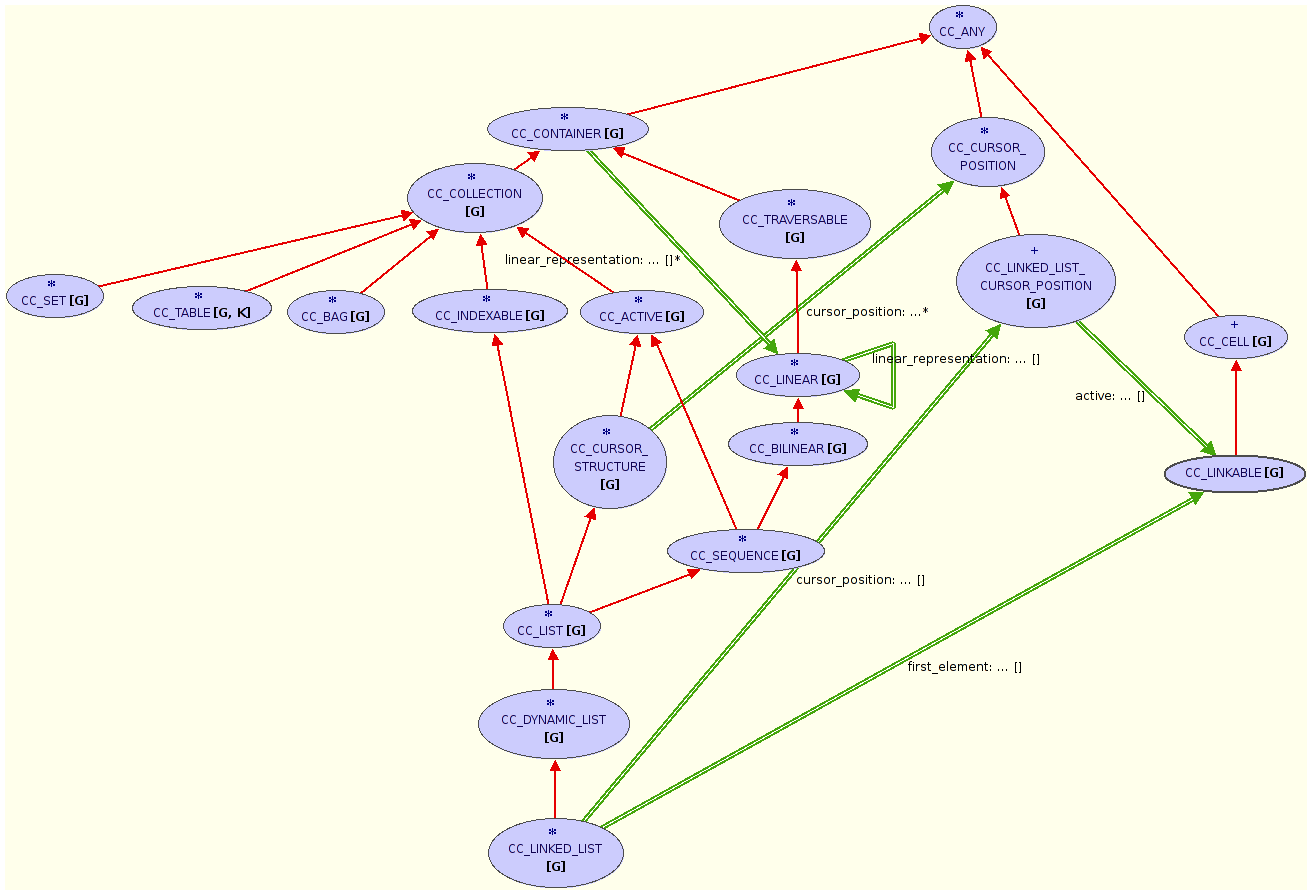
\includegraphics[width=1.00\textwidth]{pictures/CC_EiffelBase.png}
	\caption{Overview over all classes in the new EiffelBase Library with complete contracts.}
	\label{fig:CC_EiffelBase}
\end{figure}

